\usubsection{Incremento 4: Plataforma social del entorno}

El objetivo principal de este cuarto incremento fue consolidar el ecosistema del lenguaje, transformándolo de una herramienta de programación aislada a una plataforma social y colaborativa que brindara soporte a la base colaborativa de la formación del pensamiento computacional. Se recogieron, además, necesidades relacionadas con la mejora de la usabilidad del editor visual, la ampliación de la integración con hardware externo para abrir paso a la exploración de conceptos de Internet de las Cosas (IoT), y la actualización de la identidad gráfica y del catálogo de nodos.

Se organizó el trabajo del incremento en cinco líneas de desarrollo:

\begin{itemize}
  \item La construcción de una plataforma social basada en gestión de usuarios y proyectos con soporte para compartición y remezcla.
  \item La implementación de un sistema de extensiones para encapsular y compartir nodos personalizados.
  \item La integración de sensores y pines del micro:bit para habilitar escenarios de IoT.
  \item El diseño de un sistema de niveles de abstracción en la paleta de nodos.
  \item La consolidación de la identidad gráfica de la plataforma.
\end{itemize}

La necesidad de una plataforma social se fundamentó teóricamente en las observaciones de \citeA[p.~65]{resnicketal2009}, quienes destacan la importancia fundamental de dotar a un lenguaje de programación de una \emph{literatura} rica y accesible. A diferencia de enfoques anteriores (Resnick hacía referencia al lenguaje \emph{Logo} desarrollado por Papert) que carecían de ecosistemas para compartir código fácilmente, la presente plataforma permite a los niños y jóvenes estudiar técnicas de programación explorando las creaciones de otros, modificándolas y construyendo sobre ellas. Este ciclo de compartir y remezclar consolida el pensamiento computacional a través de la colaboración dentro y fuera del aula.

Por otra parte, el sistema de niveles de abstracción se planificó con una doble motivación pedagógica. En primer lugar, actúa como mecanismo de gestión de complejidad para usuarios principiantes, reduciendo la cantidad de herramientas visibles en etapas tempranas. Este principio se alinea con los hallazgos de \citeA{bers2023} en el diseño de ScratchJr, donde la limitación deliberada de comandos disponibles permitió focalizar la atención cognitiva del usuario en la lógica del problema y no en la exploración de herramientas. En segundo lugar, el sistema constituye una herramienta didáctica en manos del docente: el educador puede proponer a sus estudiantes que resuelvan un problema desde el nivel más alto de abstracción, empleando nodos que encapsulan operaciones complejas en bloques simples, y luego reducir el nivel disponible para que reconstruyan la solución a partir de primitivas más granulares. Esta dinámica funciona como un andamiaje inverso que no incrementa la dificultad del problema en sí, sino que profundiza la comprensión de los mecanismos subyacentes y fomenta la creatividad en la búsqueda de soluciones alternativas, consolidando así la práctica computacional de la abstracción y la modularización identificada por \citeA{brennan2012}.

Se modeló la plataforma social con soporte tanto para cuentas registradas como para uso anónimo mediante cookies, garantizando privacidad y reduciendo barreras de entrada. La lógica de compartición y remezcla de proyectos se diseñó siguiendo el concepto de \emph{remix} utilizado por Scratch, y se complementó con un sistema de extensiones para encapsular subflujos reutilizables en paquetes independientes. Se definió una API RESTful para la gestión de usuarios, proyectos y extensiones, soportada por una base de datos Postgres cuyo diagrama de entidad-relación se muestra en la figura \ref{fig:erd}.

Para la integración de sensores, se planificó una actualización del protocolo de distribución implementado en el segundo incremento, permitiendo al micro:bit leer su sensor de temperatura integrado y emitir valores de vuelta al cliente web, además de la lectura y escritura en los pines de las tarjetas en formato digital y analógico.

El sistema de niveles de abstracción se diseñó para permitir al usuario alternar entre tres niveles de complejidad creciente, determinando dinámicamente el subconjunto de nodos disponibles: a medida que se incrementa el nivel, se incorporan herramientas más potentes y abstractas, mientras que se ocultan los nodos más elementales.

Como parte de la consolidación de la herramienta, se planteó una reestructuración de su identidad gráfica y conceptual. La plataforma pasó a denominarse oficialmente ``NodeLand''. Esta elección encuentra su justificación teórica en el concepto de ``MathLand'' introducido por \citeA{mindstorms1980}, quien argumenta que, así como aprender francés es un proceso natural para un niño que vive en Francia y lo asimila en su día a día, el aprendizaje de las matemáticas y la computación debería ser igualmente intuitivo si el aprendiz habita un entorno donde la comunicación computacional es un lenguaje vivo y natural.

\begin{figure}[H]
    \centering
    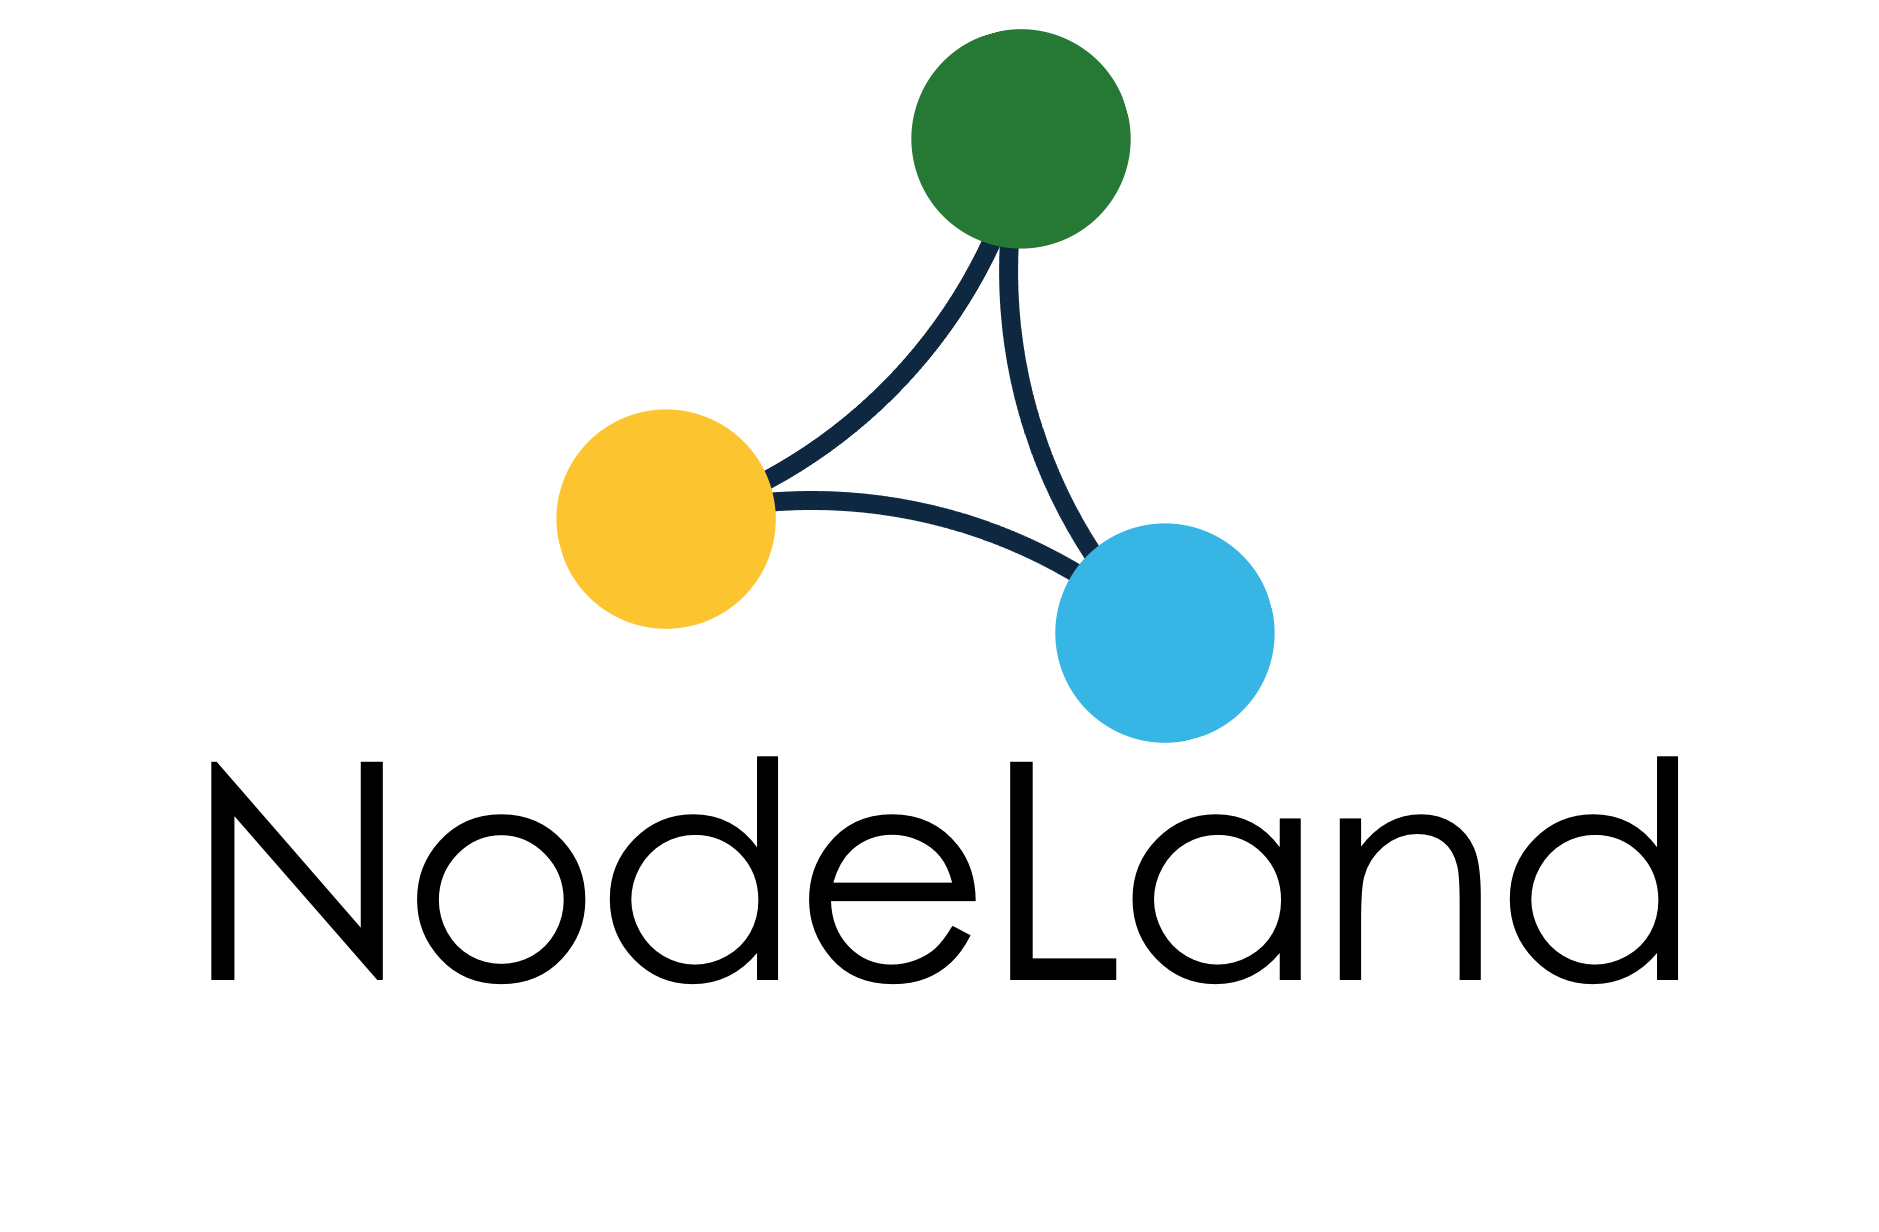
\includegraphics[width=0.4\textwidth]{../images/NodeLand.png}
    \caption[Logotipo de NodeLand]{\normalfont Logotipo de NodeLand}
    \label{fig:nodeland-logo}
\end{figure}

Siguiendo esta premisa, ``NodeLand'' (Tierra de Nodos) se concibe como un entorno inmersivo donde los niños y jóvenes pueden asimilar el paradigma de dataflow, la concurrencia y la programación interactuando en su propio ecosistema colaborativo. En la figura \ref{fig:nodeland-logo} se muestra el logotipo final de la plataforma.


La API se desarrolló con Node.js y Express, integrada con la base de datos Postgres según el modelo definido. Se implementó el flujo completo de registro, autenticación y almacenamiento de proyectos en la nube, así como la gestión anónima de proyectos mediante cookies para usuarios no registrados. La funcionalidad de compartición y remezcla se materializó según el modelo diseñado, y el sistema de extensiones se implementó permitiendo guardar, compartir e incorporar dinámicamente paquetes de nodos temáticos o funcionales al entorno de desarrollo para operar junto con los nodos nativos del sistema.

En cuanto a la integración con hardware, se implementó el nodo \emph{Leer Temperatura} para las tarjetas micro:bit, lo que requirió actualizar el protocolo de distribución para que el micro:bit emita valores de vuelta al cliente web a través de la conexión Serial o Bluetooth. Posteriormente, se implementaron nodos específicos para la lectura y escritura en los pines del micro:bit en formato digital y analógico, abriendo las puertas a la integración directa de una amplia variedad de sensores y actuadores externos. La incorporación de estos nodos sirve como una prueba de concepto de cómo el paradigma de dataflow facilita la codificación de entornos de IoT de manera intuitiva.

El sistema de niveles de abstracción se implementó en la paleta de nodos con los tres niveles planificados. Ya consolidados todos los nodos del lenguaje con sus niveles correspondientes, se completó su documentación en un catálogo disponible en el apéndice \ref{apx:node-catalog}.

La validación se realizó mediante pruebas funcionales sobre la plataforma social y la integración con hardware. Se comprobó el correcto registro y almacenamiento de proyectos, así como su recuperación y reutilización, lo que permitió cumplir con el requerimiento de ofrecer plantillas de proyectos precargadas para usuarios tanto autenticados como anónimos. También se verificó la funcionalidad de compartir y editar proyectos dentro de la plataforma, cubriendo el requerimiento de fomentar el uso en un contexto social y colaborativo. En el componente físico, se ejecutaron pruebas de lectura de temperatura y de interacción con pines del micro:bit, confirmando la correcta transmisión de datos entre el hardware y el entorno web y consolidando la capacidad de delegación y ejecución en hardware externo.

Como resultado de este incremento, el lenguaje evolucionó hacia una plataforma integral, colaborativa y extensible cuya arquitectura basada en el navegador permite el acceso sin instalaciones. Las capacidades sociales fortalecieron la dimensión comunitaria del aprendizaje, la integración de sensores y pines amplió el potencial del sistema para proyectos de computación física, y la consolidación de la identidad bajo el nombre ``NodeLand'' reforzó la coherencia conceptual de la propuesta y su proyección como entorno educativo.